\documentclass{beamer}

\usetheme{Madrid}
\usepackage{graphicx}
\usepackage[utf8]{inputenc}  
\usepackage[T1]{fontenc}     
\usepackage{textcomp}        

\title[SKBD] {Proposal for SKBDS}

\author[Pictures]
{Barna Mikler \and Botond Geönczeöl \and Dominik Li \and \\ Mátyás Dávid \and Bálint Boros}

\institute[ELTE]{Eötvös Loránd University \\ Faculty of Informatics}

\date[2024] {November 2024}

\logo{
\includegraphics[height=1cm]{images/elte_cimer_szines.eps}}

\begin{document}

\frame{\titlepage}

\begin{frame}
\frametitle{Table of Contents}
\tableofcontents
\end{frame}  

\section{Project Overview}
\begin{frame}
\frametitle{Project Overview}
\begin{itemize}
    \item SKBD, Background
    \item Objective
    \item Development Plan
    \item Impact
    \item Advertisement
\end{itemize}
\end{frame}

\section{Project Context}
\begin{frame}
\frametitle{Project Context}
\begin{itemize}
    \item Addressed Problem
    \item Urgency, Need
\end{itemize}
\end{frame}

\section{Project Participants}
\begin{frame}
\frametitle{Project Participants}
\begin{itemize}
    \item Diverse team combining universities, research organizations, and industry partners from multiple countries.
    \item Key participants include:
    \begin{itemize}
        \item \textbf{Eötvös Loránd University (Hungary)}
        \item \textbf{Charles University (Czech Republic)}
        \item \textbf{Grenoble Alpes University (France)}
        \item \textbf{IT University of Copenhagen (Denmark)}
        \item \textbf{Nokia Corporation (Finland)}
        \item \textbf{Lexunit Group Ltd. (Hungary)}
    \end{itemize}
    \item Collaboration ensures shared resources, interdisciplinary expertise, and innovative results.
\end{itemize}
\end{frame}

\section{Roles and Responsibilities}
\begin{frame}
\frametitle{Roles and Responsibilities}
\begin{itemize}
    \item \textbf{Eötvös Loránd University (ELTE)}: Manages the project and develops algorithms for room layout detection.
    \item \textbf{Charles University (KU)}: Optimizes algorithms for cuboid rooms to improve efficiency.
    \item \textbf{Grenoble Alpes University (UGA)}: Extracts spatial descriptors using Convolutional Neural Networks.
    \item \textbf{IT University of Copenhagen (ITU)}: Ensures algorithm integration and descriptor compatibility.
    \item \textbf{Nokia Corporation}: Harmonizes virtual and analogue data for accurate reconstruction.
    \item \textbf{Lexunit Group Ltd.}: Builds the user-friendly application integrating all project tools.
\end{itemize}
\end{frame}

\section{Beneficiaries}
\begin{frame}
\frametitle{Beneficiaries}
\begin{itemize}
    \item Global Scope
    \item National Scope
    \item Personal Scope
\end{itemize}
\end{frame}


% WORK PACKAGES
\section{Work Packages}
\begin{frame}
\frametitle{Work Packages}
\begin{itemize}
    \item Segment Knotting Boundary Detection (SKBD) for Room Layout Detection
    \item Optimizing SKBD for Standard Cuboid Rooms
    \item High Accuracy Virtual to Analogue Harmonization
    \item Enchanced Descriptor Extraction using CNNs
    \item End-User Application
\end{itemize}
\end{frame}

\section{WP Descriptions}
\begin{frame}
\frametitle{Work Package 1}
\textbf{Segment Knotting Boundary Detection (SKBD) for Room Layout Detection}
\begin{itemize}
    \item SKBD Algorithm
    \item SKBD Report
    \item SKBD API
\end{itemize}
\end{frame}

\begin{frame}
\frametitle{Work Package 2}
\textbf{Optimizing SKBD for Standard Cuboid Rooms}
\begin{itemize}
    \item SKBD Fine-tuning for Cuboid Rooms
    \item SKBD Algorithm-switching
    \item Optimized SKBD Report
    \item Optimized SKBD API
\end{itemize}
\end{frame}

\begin{frame}
\frametitle{Work Package 3}
\textbf{High Accuracy Virtual to Analogue Harmonization (HAV2AH)}
\begin{itemize}
    \item HAV2AH Algorithm
    \item HAV2AH Report
    \item HAV2AH SKBD Integration
    \item HAV2AH Demonstration
\end{itemize}
\end{frame}

\begin{frame}
\frametitle{Work Package 4}
\textbf{Enhanced Descriptor Extraction using CNNs}
\begin{itemize}
    \item CNN Training
    \item CNN Report
    \item CNN Integration
\end{itemize}
\end{frame}

\begin{frame}
\frametitle{Work Package 5}
\textbf{Development of End-User Application}
\begin{itemize}
    \item User App Prototype
    \item User App Full
    \item User App Report
    \item User App Documentation
    \item User App Deployment
\end{itemize}
\end{frame}

\section{Agenda and Milestones}
\begin{frame}
\frametitle{Agenda and Milestones}
\begin{figure}[htbp]
    \centering
    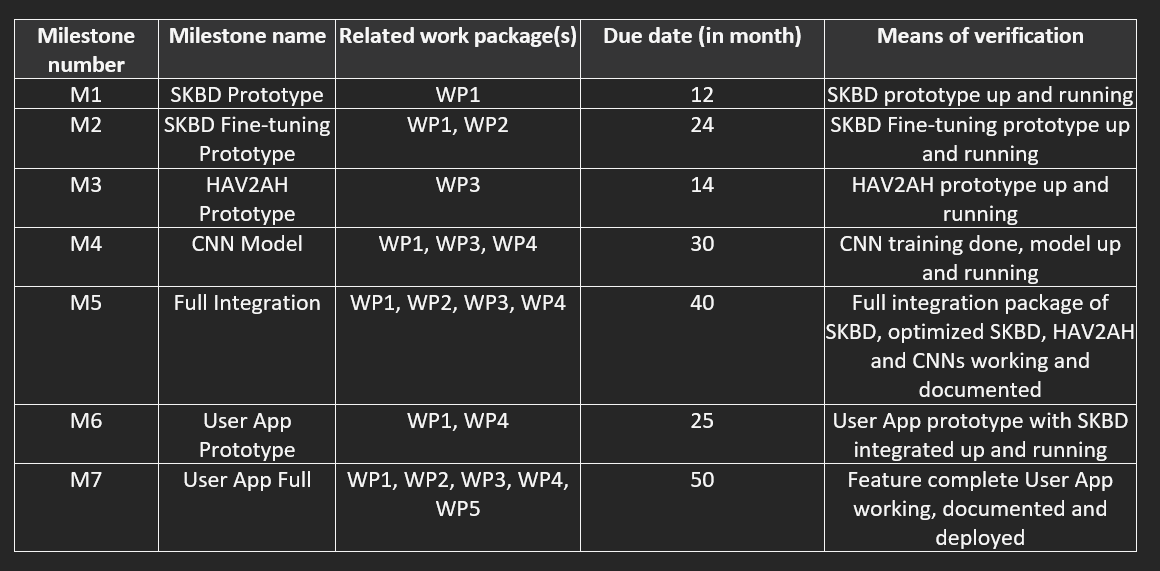
\includegraphics[width=1\textwidth]{images/milestones.png}
    \caption{Project Milestones Overview}
    \label{fig:milestones}
\end{figure}
\end{frame}

\section{Gantt Chart}
\begin{frame}
\frametitle{Gantt Chart}
\begin{figure}[htbp]
    \centering
    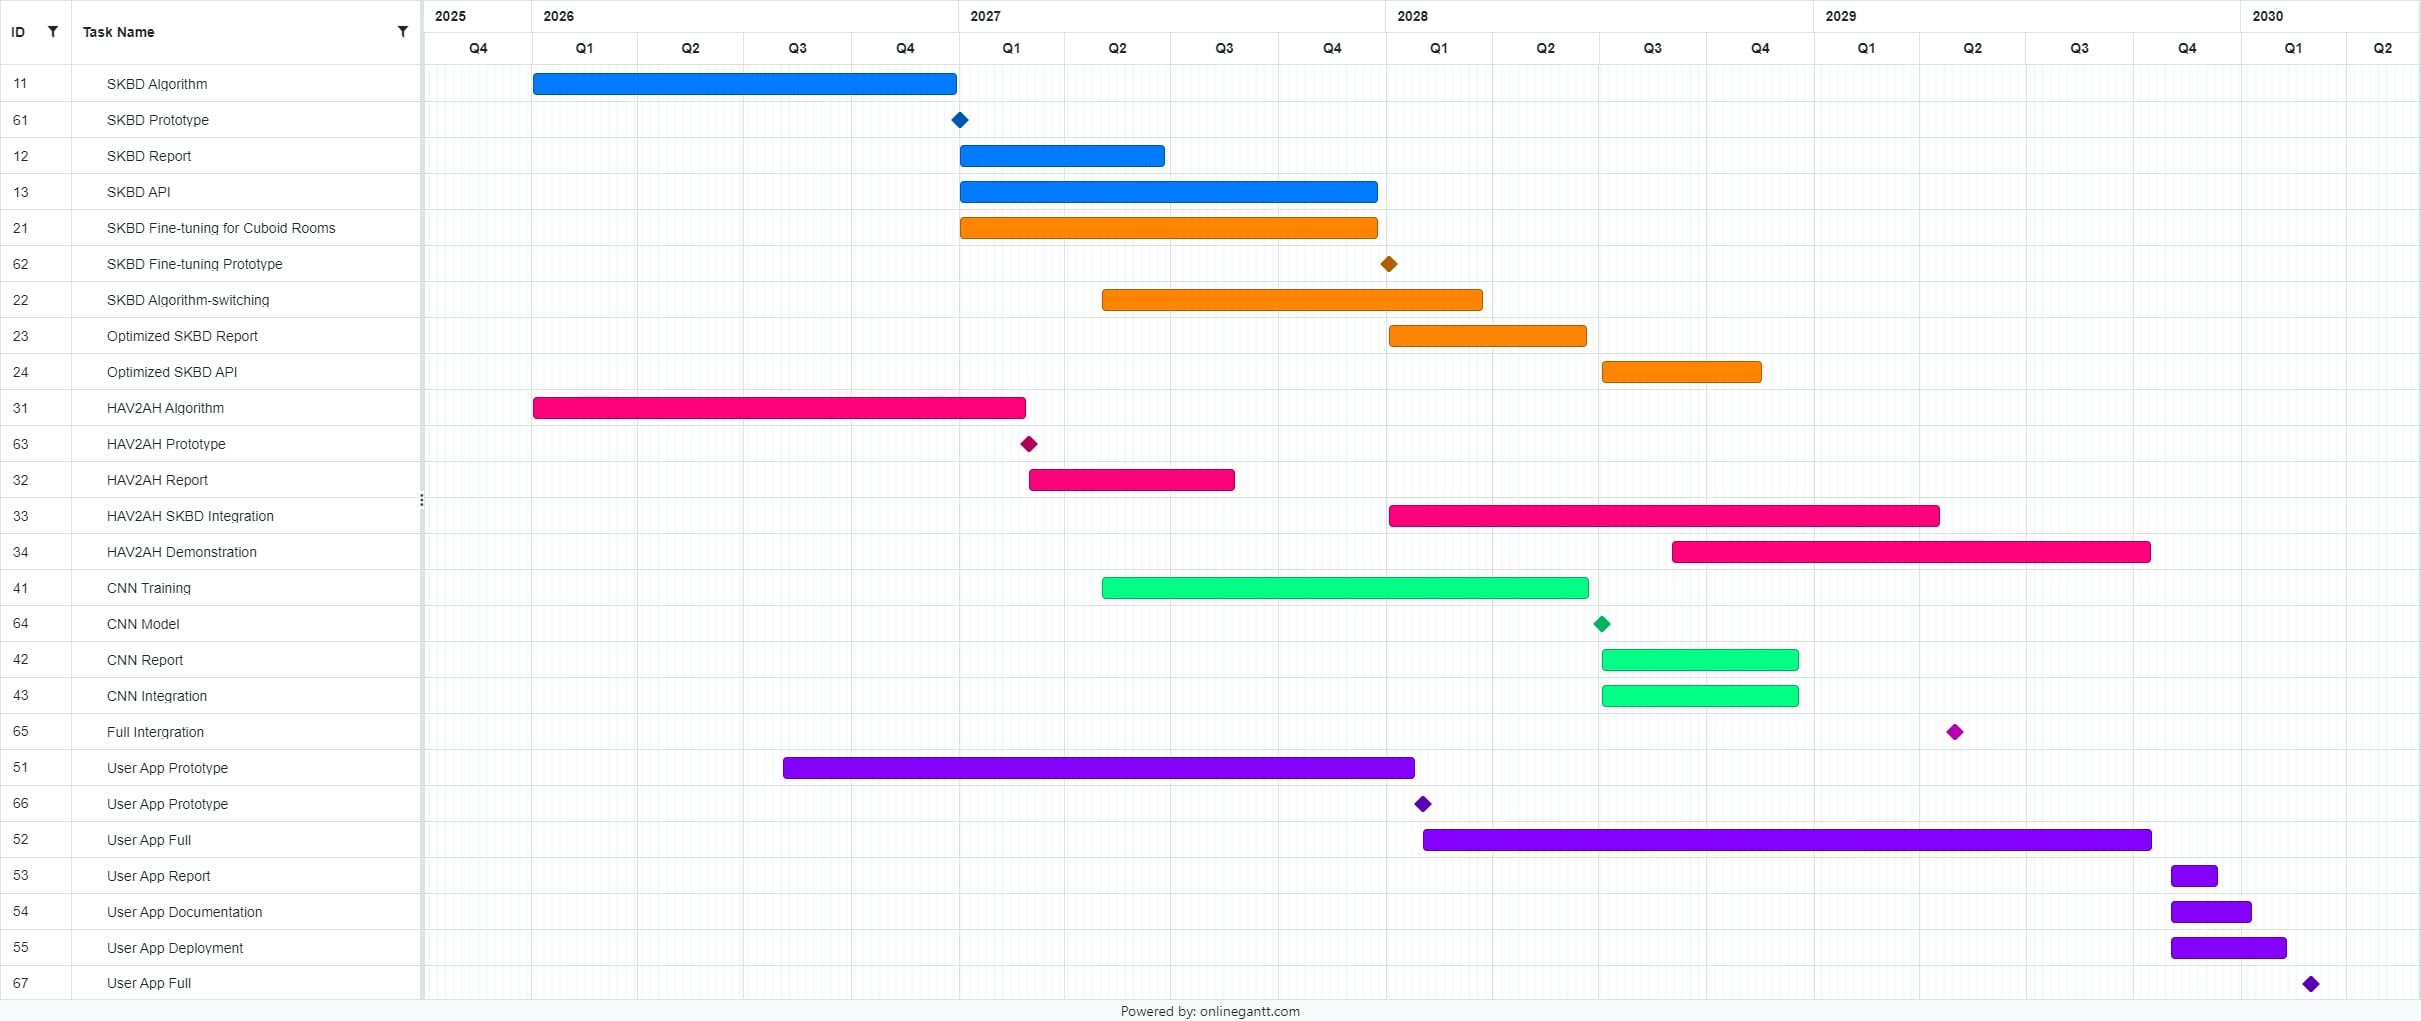
\includegraphics[width=1\textwidth]{images/gant.jpg}
    \caption{Project Gantt diagram}
    \label{fig:gantt}
\end{figure}

\end{frame}

\section{Budget Breakdown}
\begin{frame}
\frametitle{Budget Breakdown}

\begin{figure}[htbp]
    \centering
    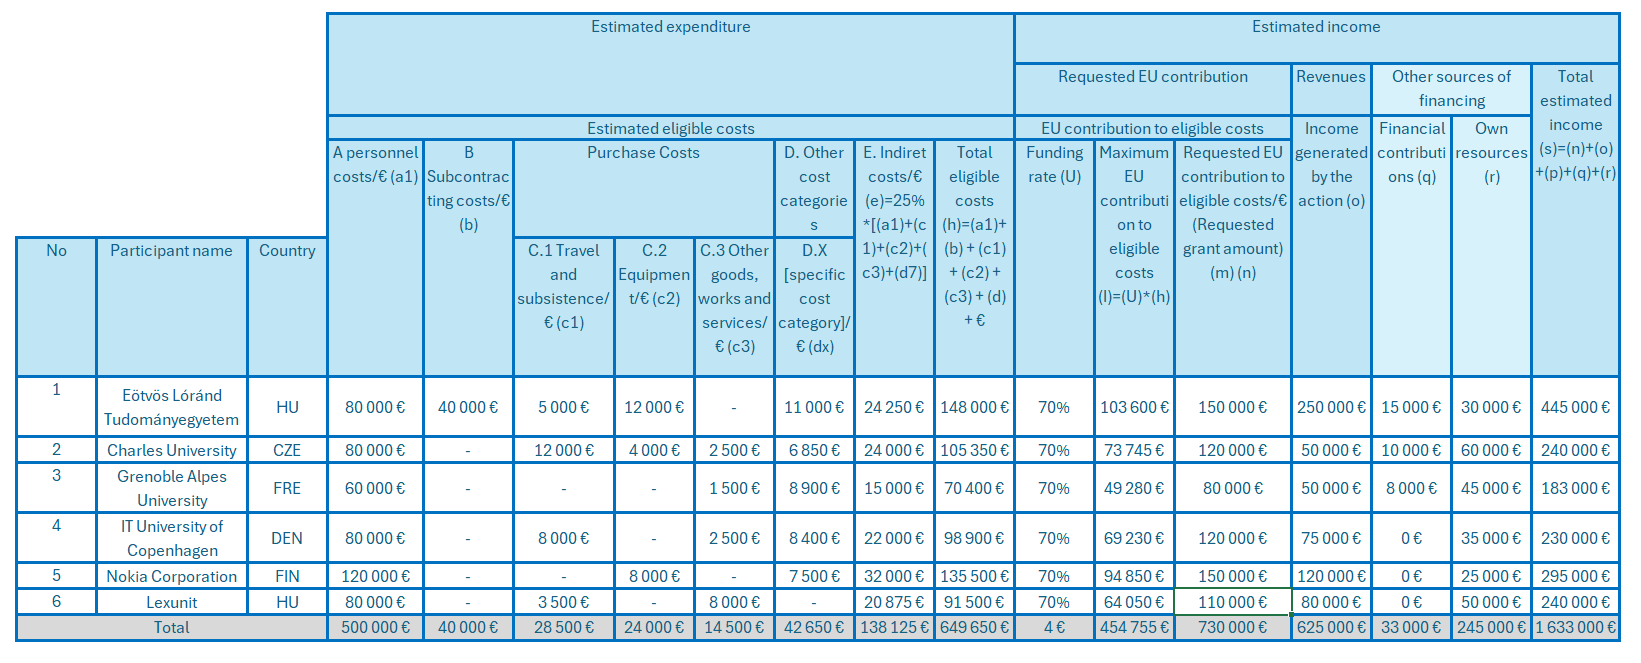
\includegraphics[width=1\textwidth]{images/budget.png}
    \caption{Project Budget Overview}
    \label{fig:budget}
\end{figure}

\end{frame}

\section{Levels of Risks}
\begin{frame}
\frametitle{Levels of Risks}

\begin{itemize}
    \item Developing a non well rounded solution (WP1, WP2)
    \item HAV2AH not being integrateable into the solution (WP3)
    \item CNN training more expensive than forecasted (WP4)
    \item Beta testing takes longer than anticipated (WP5)
\end{itemize}

\end{frame}

\section{Ethics}
\begin{frame}
\frametitle{Ethics}
\begin{itemize}
    \item The project fully complies with EU ethical standards, including the European Code of Conduct for Research Integrity and GDPR.
    \item Ethical considerations include the use of synthetic and publicly available datasets to avoid personal data concerns.
    \item The project employs Convolutional Neural Networks (CNNs) for computational tasks, ensuring transparency and responsible use of AI technologies.
    \item Balances scientific innovation with societal and ethical responsibilities.
\end{itemize}
\end{frame}

\section{Impact and Dissemination}
\begin{frame}
\frametitle{Impact and Dissemination}
    Impact
    \begin{itemize}
        \item Foundational
        \item Economical
    \end{itemize}
    Dissemination Measures
    \begin{itemize}
        \item Dissemination: Scientific publications
        \item Exploitation: Patenting
        \item Communication: Offers, Website, Adverisements
    \end{itemize}
\end{frame}

\section{Conclusion}
\begin{frame}
\frametitle{Conclusion}
\begin{itemize}
     \item Advancing the field of digital reconstruction
     \item Efficient, precise, and scalable solution
     \item Aligns perfectly with the Horizon Europe program’s goals for innovation and societal impact
\end{itemize}
\end{frame}

\section{QA}
\begin{frame}
\frametitle{QA}
QA
\end{frame}

\end{document}
